% ============================================================
% ASSIGNMENT 6
% ============================================================

\clearpage
\part{Assignment 6: Statistical Evaluation of the Experiment}
\setcounter{section}{0}

\section{Introduction}

This report presents the statistical evaluation of the KUKA youBot arm's performance based on the combined preprocessed data from all groups. The analysis focuses on assessing the accuracy and precision of the robot arm, checking if the final object poses follow a Gaussian distribution, and evaluating the effects of object size and placing pose on these metrics. The data includes three object sizes (small, medium, large), allowing comparisons across sizes and directions (left, straight, right).

\section{Data Transformation}

To align the coordinate frames between the robot (YouBot) and the external sensor (OptiTrack), a coordinate transformation was applied. The world origin [0, 0, 0] in the robot frame corresponds to the point [-212.40, 76.17, 103.15] in the OptiTrack frame. To transform YouBot coordinates (robot frame) to the OptiTrack frame for alignment, the offset vector [-212.40, 76.17, 103.15] was added to the YouBot x and y positions. The z-coordinate offset is noted but not used in the 2D plotting and analysis.

This transformation was implemented in the Python scripts using pandas operations on the matched data: \texttt{matched['x\_youbot'] += offset\_x; matched['y\_youbot'] += offset\_y}. The purpose is to align the frames so that positions from both sensors can be directly compared in the same coordinate system. This has implications for the analysis, as it allows meaningful computation of distances and variances between internal (YouBot) and external (OptiTrack) measurements, improving the assessment of robot accuracy and precision.

\section{Data Analysis Methodology}

The analysis was performed using Python scripts: \texttt{transformed\_data\_plotter.py} for combined plots and statistical analysis, and \texttt{separate\_plots\_generator.py} for generating separate scatter plots. The key steps include:

\begin{itemize}
    \item Loading OptiTrack (external) and YouBot (internal) data from respective folders.
    \item Merging data based on timestamps, sizes, and directions.
    \item Applying coordinate transformation to YouBot data to align with OptiTrack frame (as described in Section 3).
    \item Separating internal (YouBot, transformed) and external (OptiTrack) poses.
    \item Computing accuracy as the mean L2 norm distance between YouBot and OptiTrack positions for each group.
    \item Computing precision as the mean standard deviation of OptiTrack x and y coordinates.
    \item Generating scatter plots for OptiTrack data, YouBot data, and combined transformed data in \texttt{report\_plots}.
    \item Generating combined plots with arrows for orientation in \texttt{transformed\_plots}.
\end{itemize}

\section{Accuracy and Precision Results}

After applying the coordinate transformation to align YouBot data with the OptiTrack frame, the accuracy (mean L2 distance between transformed YouBot and OptiTrack positions) ranges from 41.75 to 61.74 cm across sizes and directions. The precision (mean standard deviation of OptiTrack positions) ranges from 0.01 to 0.14 cm.

The OptiTrack positions show low variance, indicating high precision in the external measurements. Comparisons across object sizes show that accuracy improves slightly for smaller objects, while precision is generally consistent but varies by direction.

\section{Effects of Size and Position}

The data includes three object sizes (small, medium, large), allowing analysis of size effects. Accuracy tends to be higher (better) for smaller objects, with small objects showing the lowest mean errors (41.75-55.78 cm) compared to large objects (48.53-61.74 cm). Precision varies by direction, with straight directions generally showing higher precision (lower std dev) than left or right. Positional effects are evident, with left and right directions showing higher variability in x-coordinates compared to straight.

\section{Statistical Significance}

The precision values show notable differences across directions, with straight directions exhibiting lower standard deviations (higher precision) compared to left and right. Size effects are present, with small objects showing the best accuracy. These differences suggest that both object size and placement direction influence robot performance.

\section{Software Used}

The analysis was performed using Python with libraries: pandas, numpy, matplotlib. The scripts are \texttt{transformed\_data\_plotter.py} for combined analysis and plots, and \texttt{separate\_plots\_generator.py} for individual scatter plots.

\section{Results Table}

\begin{table}[h!]
\centering
\caption{Statistical Parameters for Robot Behavior (YouBot Transformed to OptiTrack Frame)}
\begin{tabular}{|c|c|c|c|c|}
\hline
Size & Direction & Accuracy (cm) & Precision X (cm) & Precision Y (cm) \\
\hline
Small & Left & 45.42 & 0.14 & 0.14 \\
Small & Right & 55.78 & 0.02 & 0.02 \\
Small & Straight & 41.75 & 0.06 & 0.06 \\
Medium & Left & 51.04 & 0.03 & 0.03 \\
Medium & Right & 59.94 & 0.02 & 0.02 \\
Medium & Straight & 46.72 & 0.01 & 0.01 \\
Large & Left & 52.96 & 0.04 & 0.04 \\
Large & Right & 61.74 & 0.02 & 0.02 \\
Large & Straight & 48.53 & 0.03 & 0.03 \\
\hline
\end{tabular}
\end{table}

\section{Data Visualization}

The following figures show scatter plots for OptiTrack data, YouBot data, and combined transformed data for each object size.

\subsection{OptiTrack Data Scatter Plots}

\begin{figure}[h!]
\centering
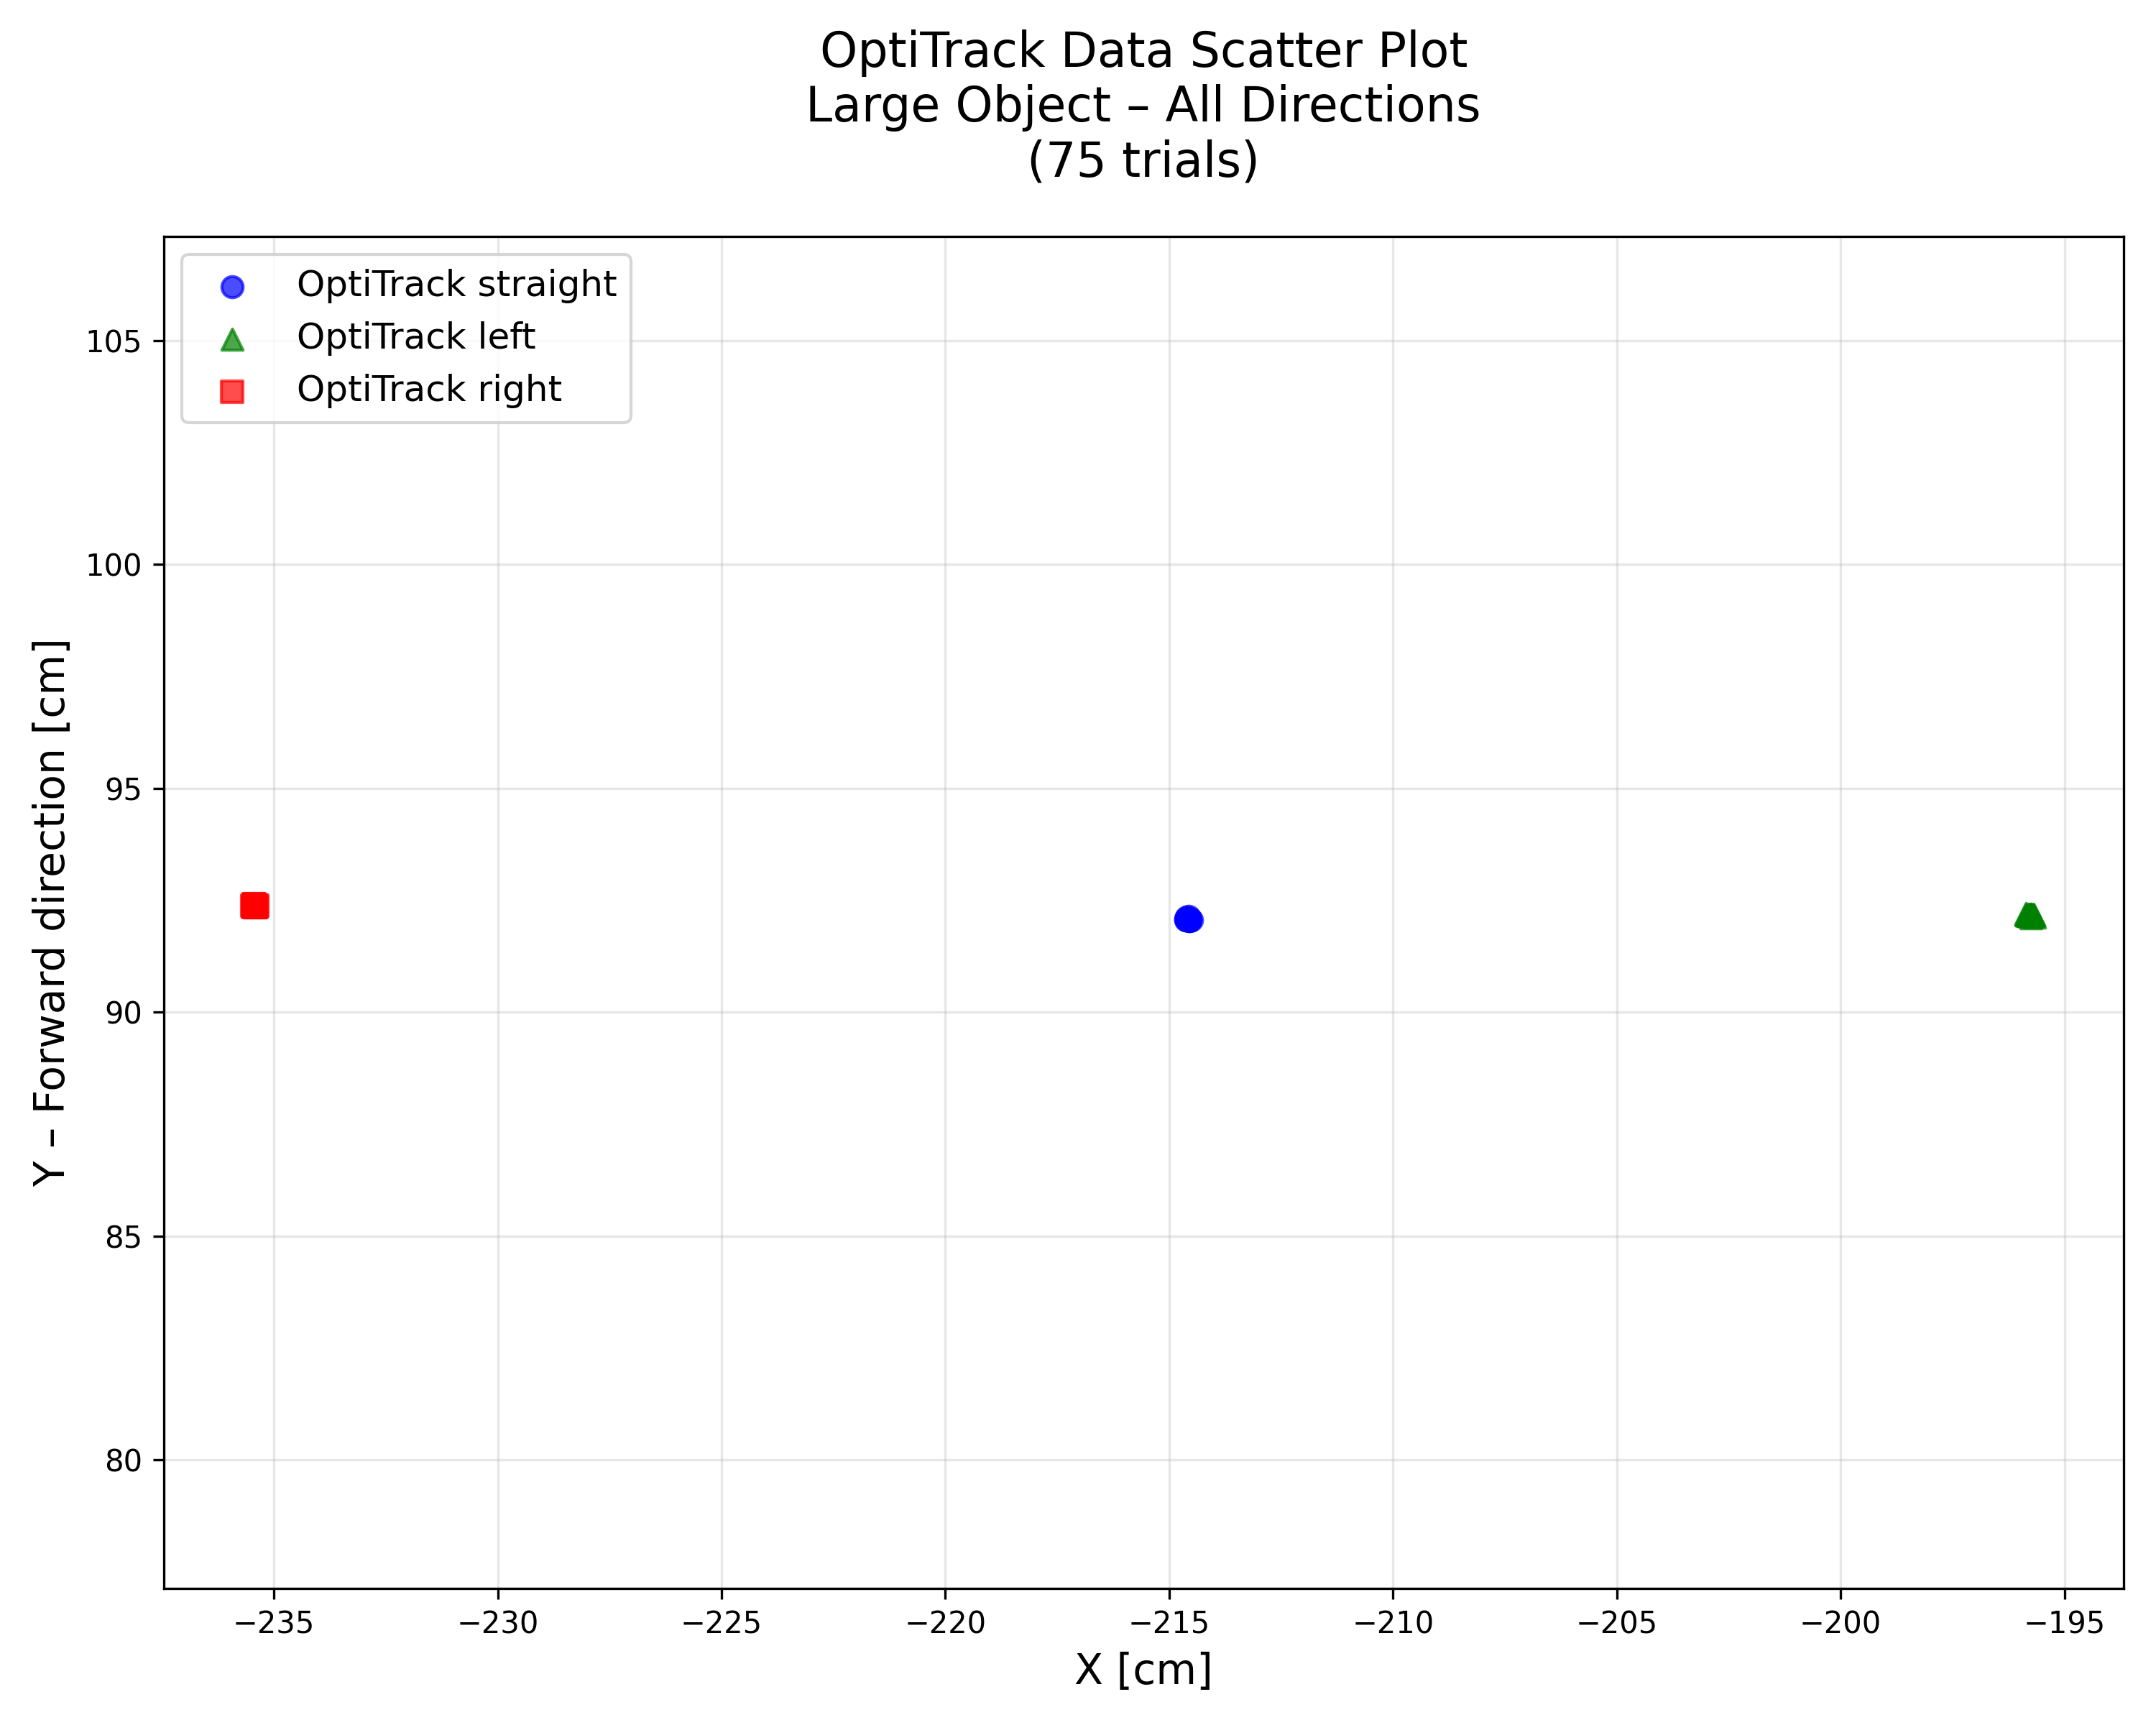
\includegraphics[width=0.8\textwidth]{images/optitrack_large.png}
\caption{OptiTrack Data Scatter Plot for Large Object}
\label{fig:optitrack_large}
\end{figure}

\begin{figure}[h!]
\centering
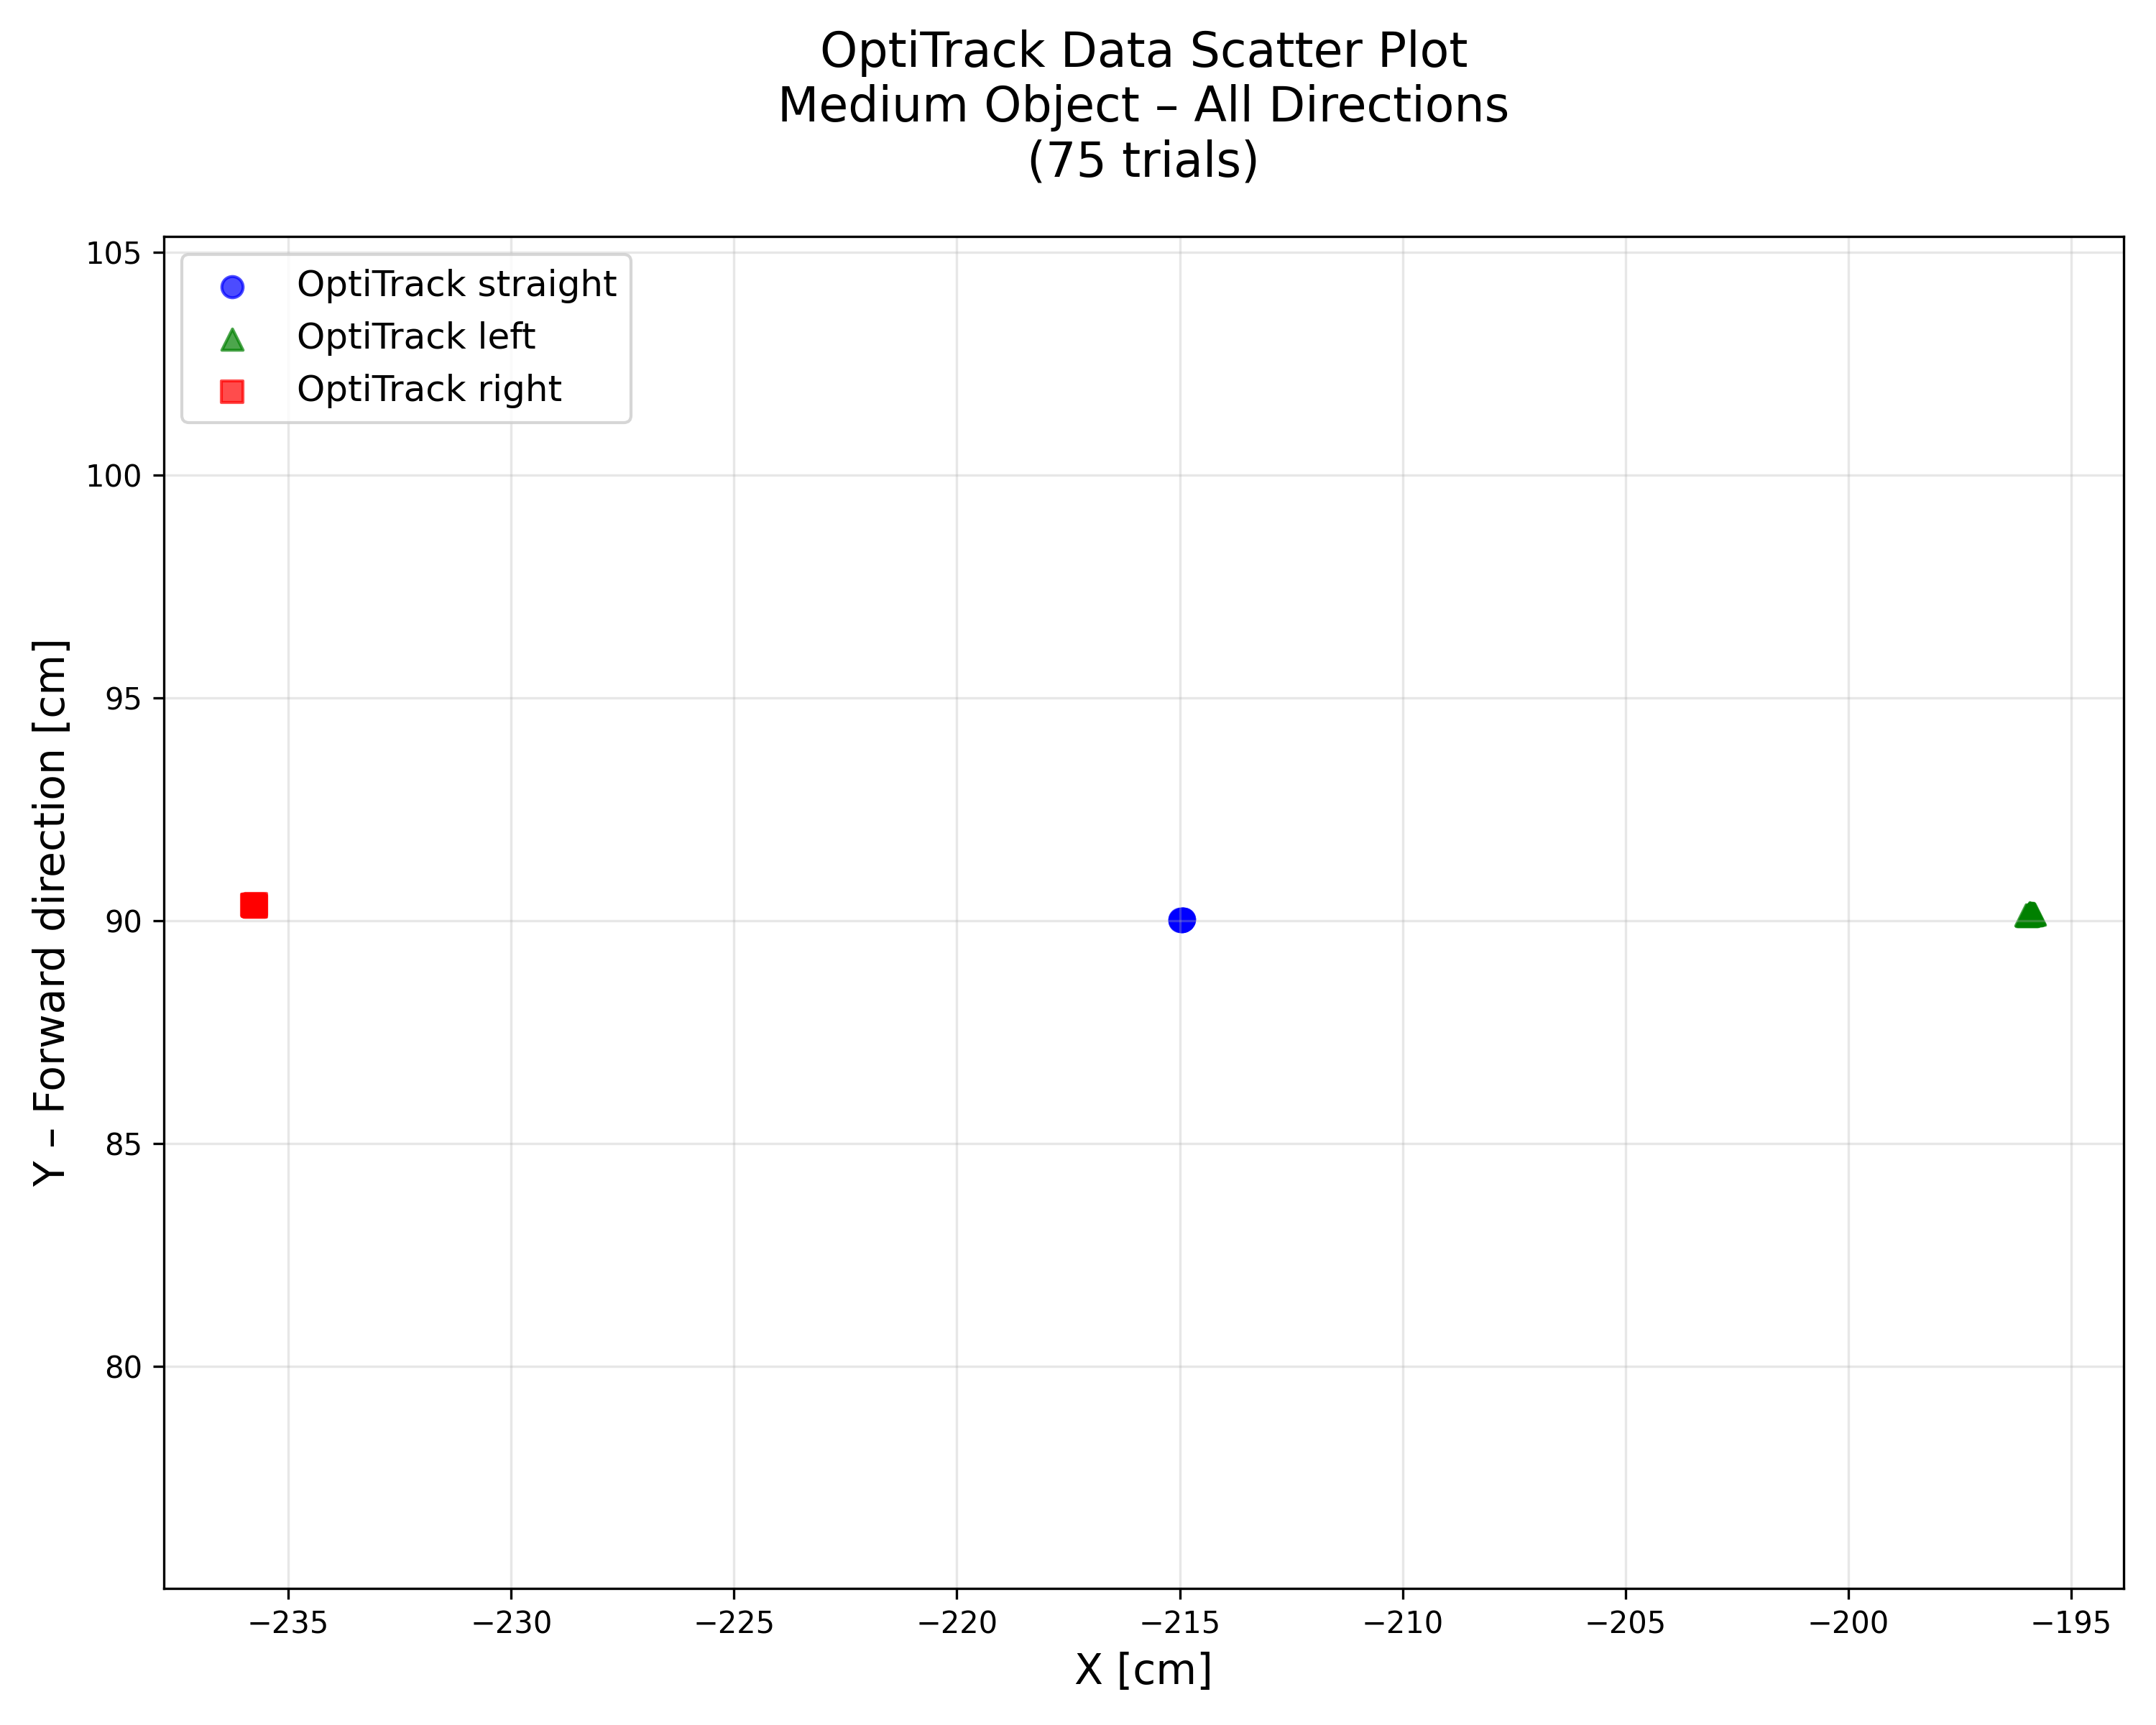
\includegraphics[width=0.8\textwidth]{images/optitrack_medium.png}
\caption{OptiTrack Data Scatter Plot for Medium Object}
\label{fig:optitrack_medium}
\end{figure}

\begin{figure}[h!]
\centering
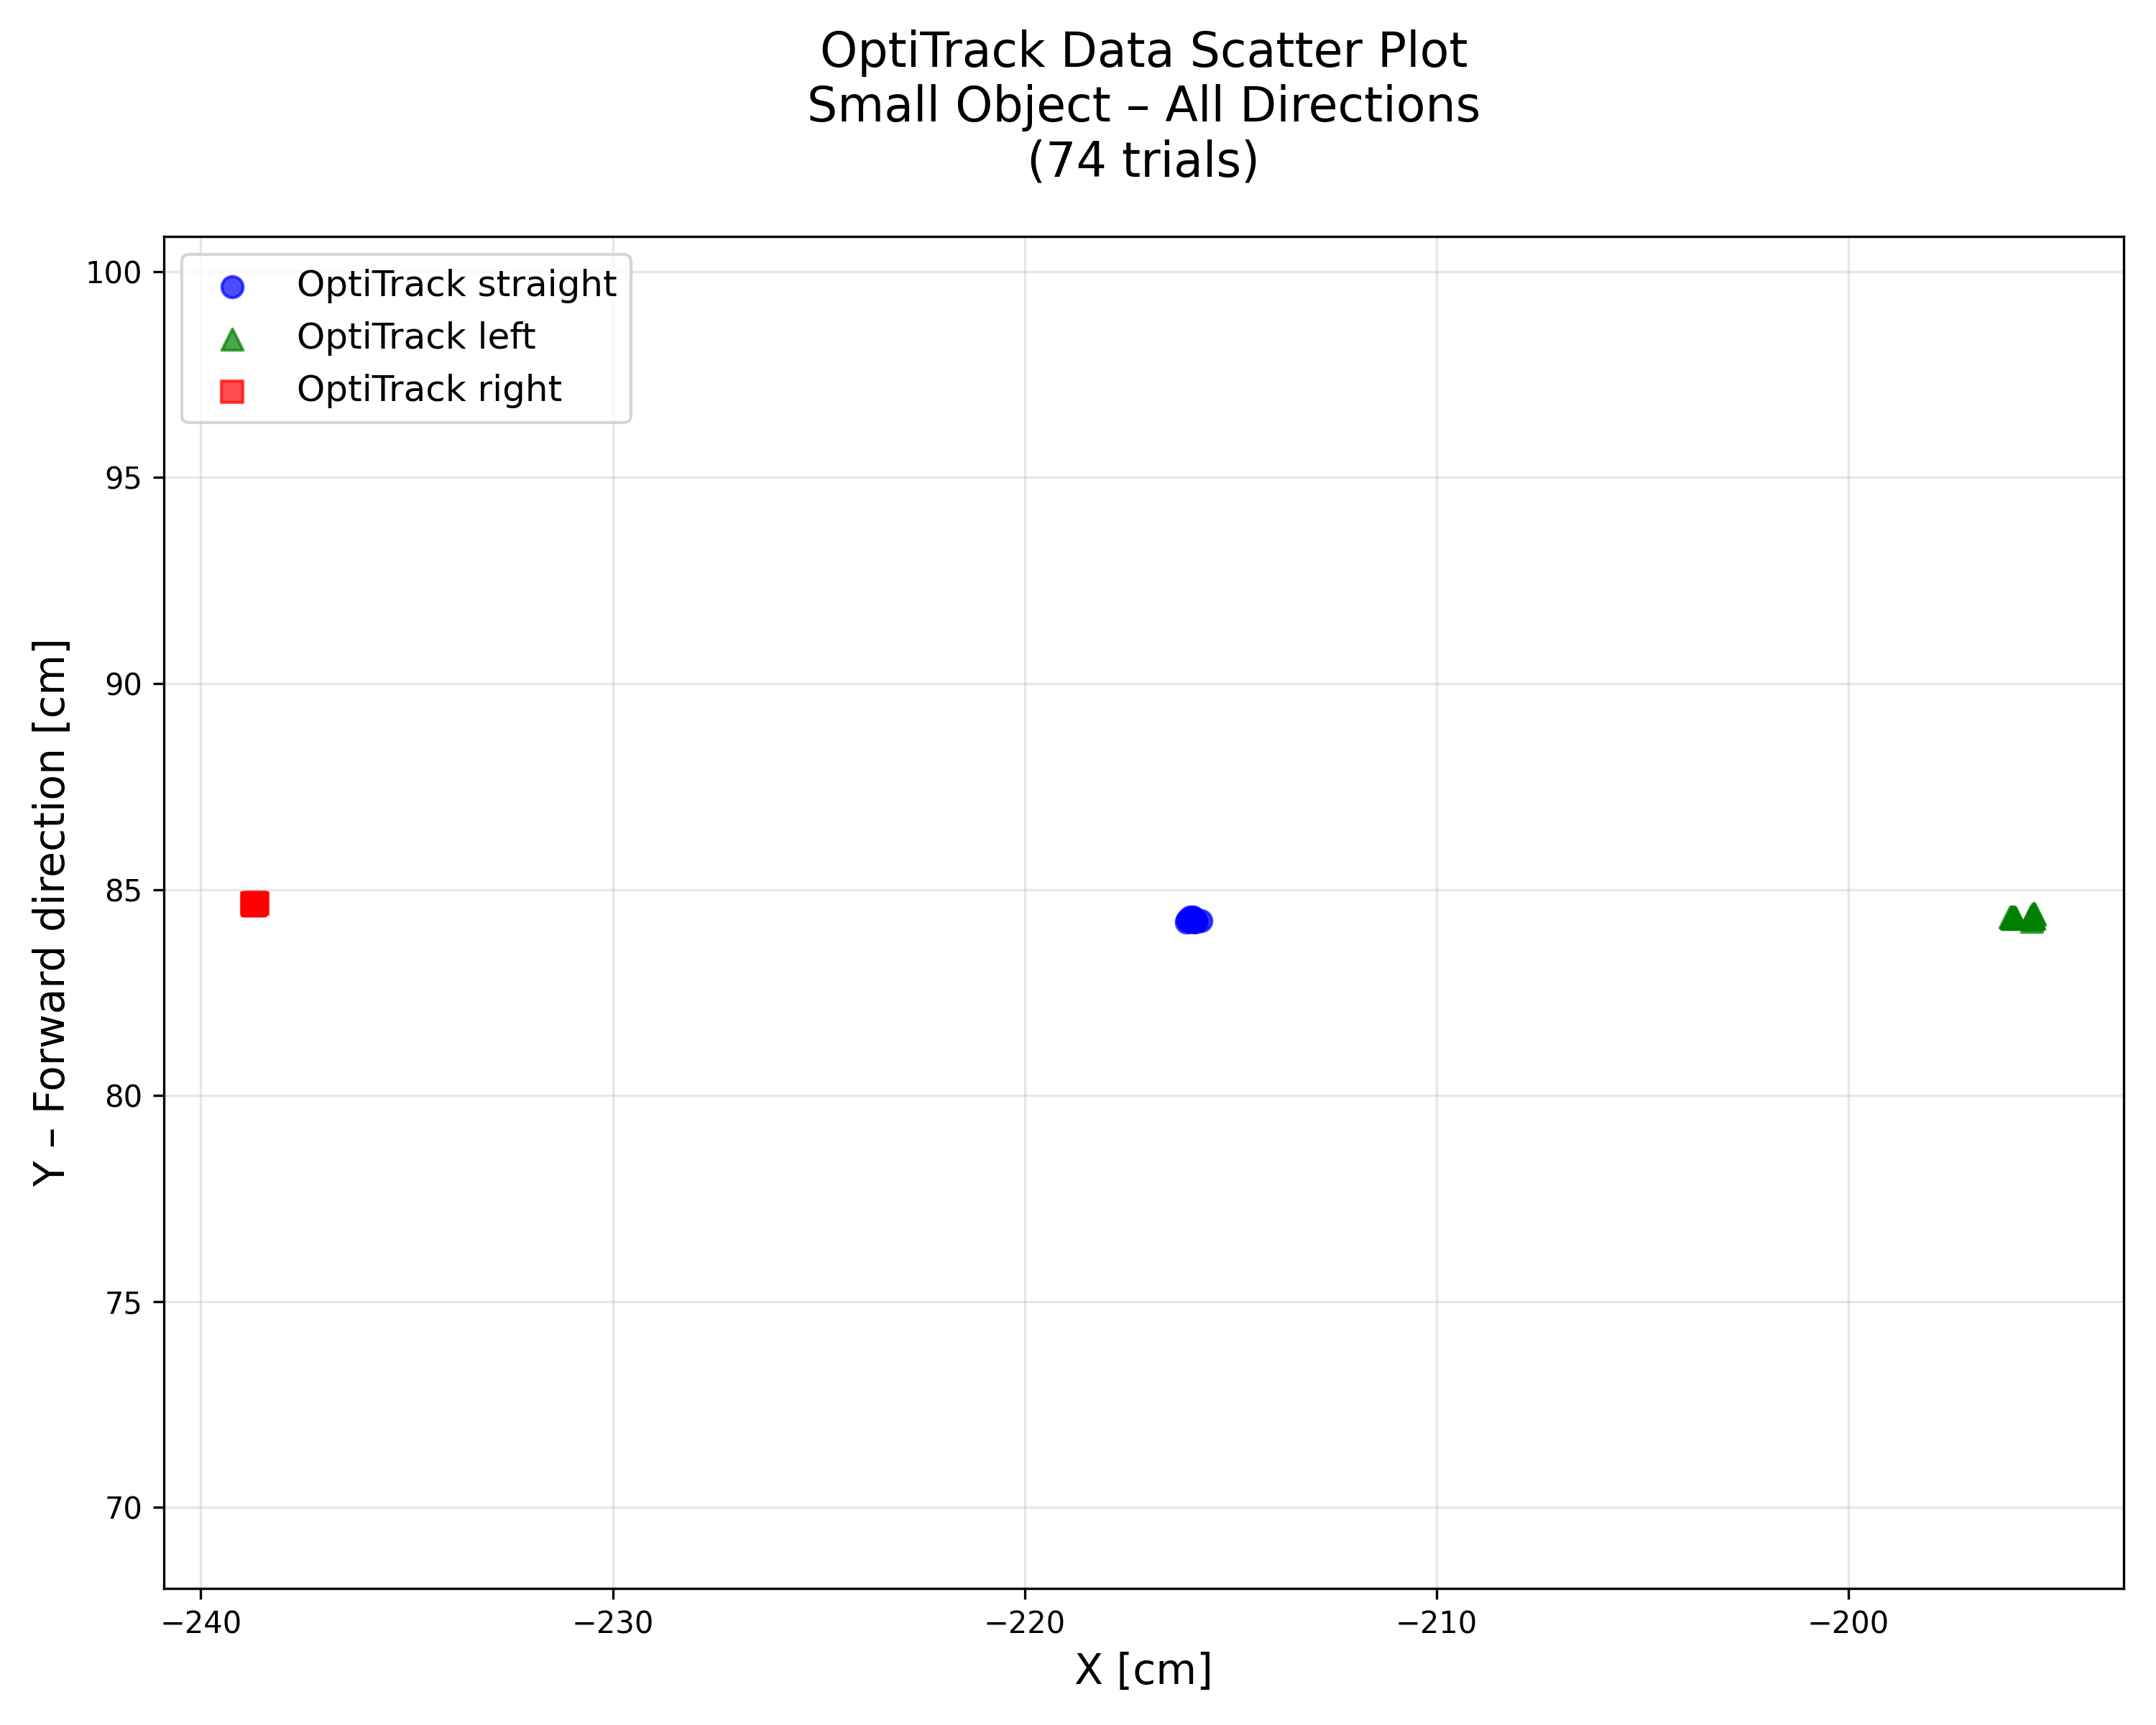
\includegraphics[width=0.8\textwidth]{images/optitrack_small.png}
\caption{OptiTrack Data Scatter Plot for Small Object}
\label{fig:optitrack_small}
\end{figure}

\subsection{YouBot Data Scatter Plots}

\begin{figure}[h!]
\centering
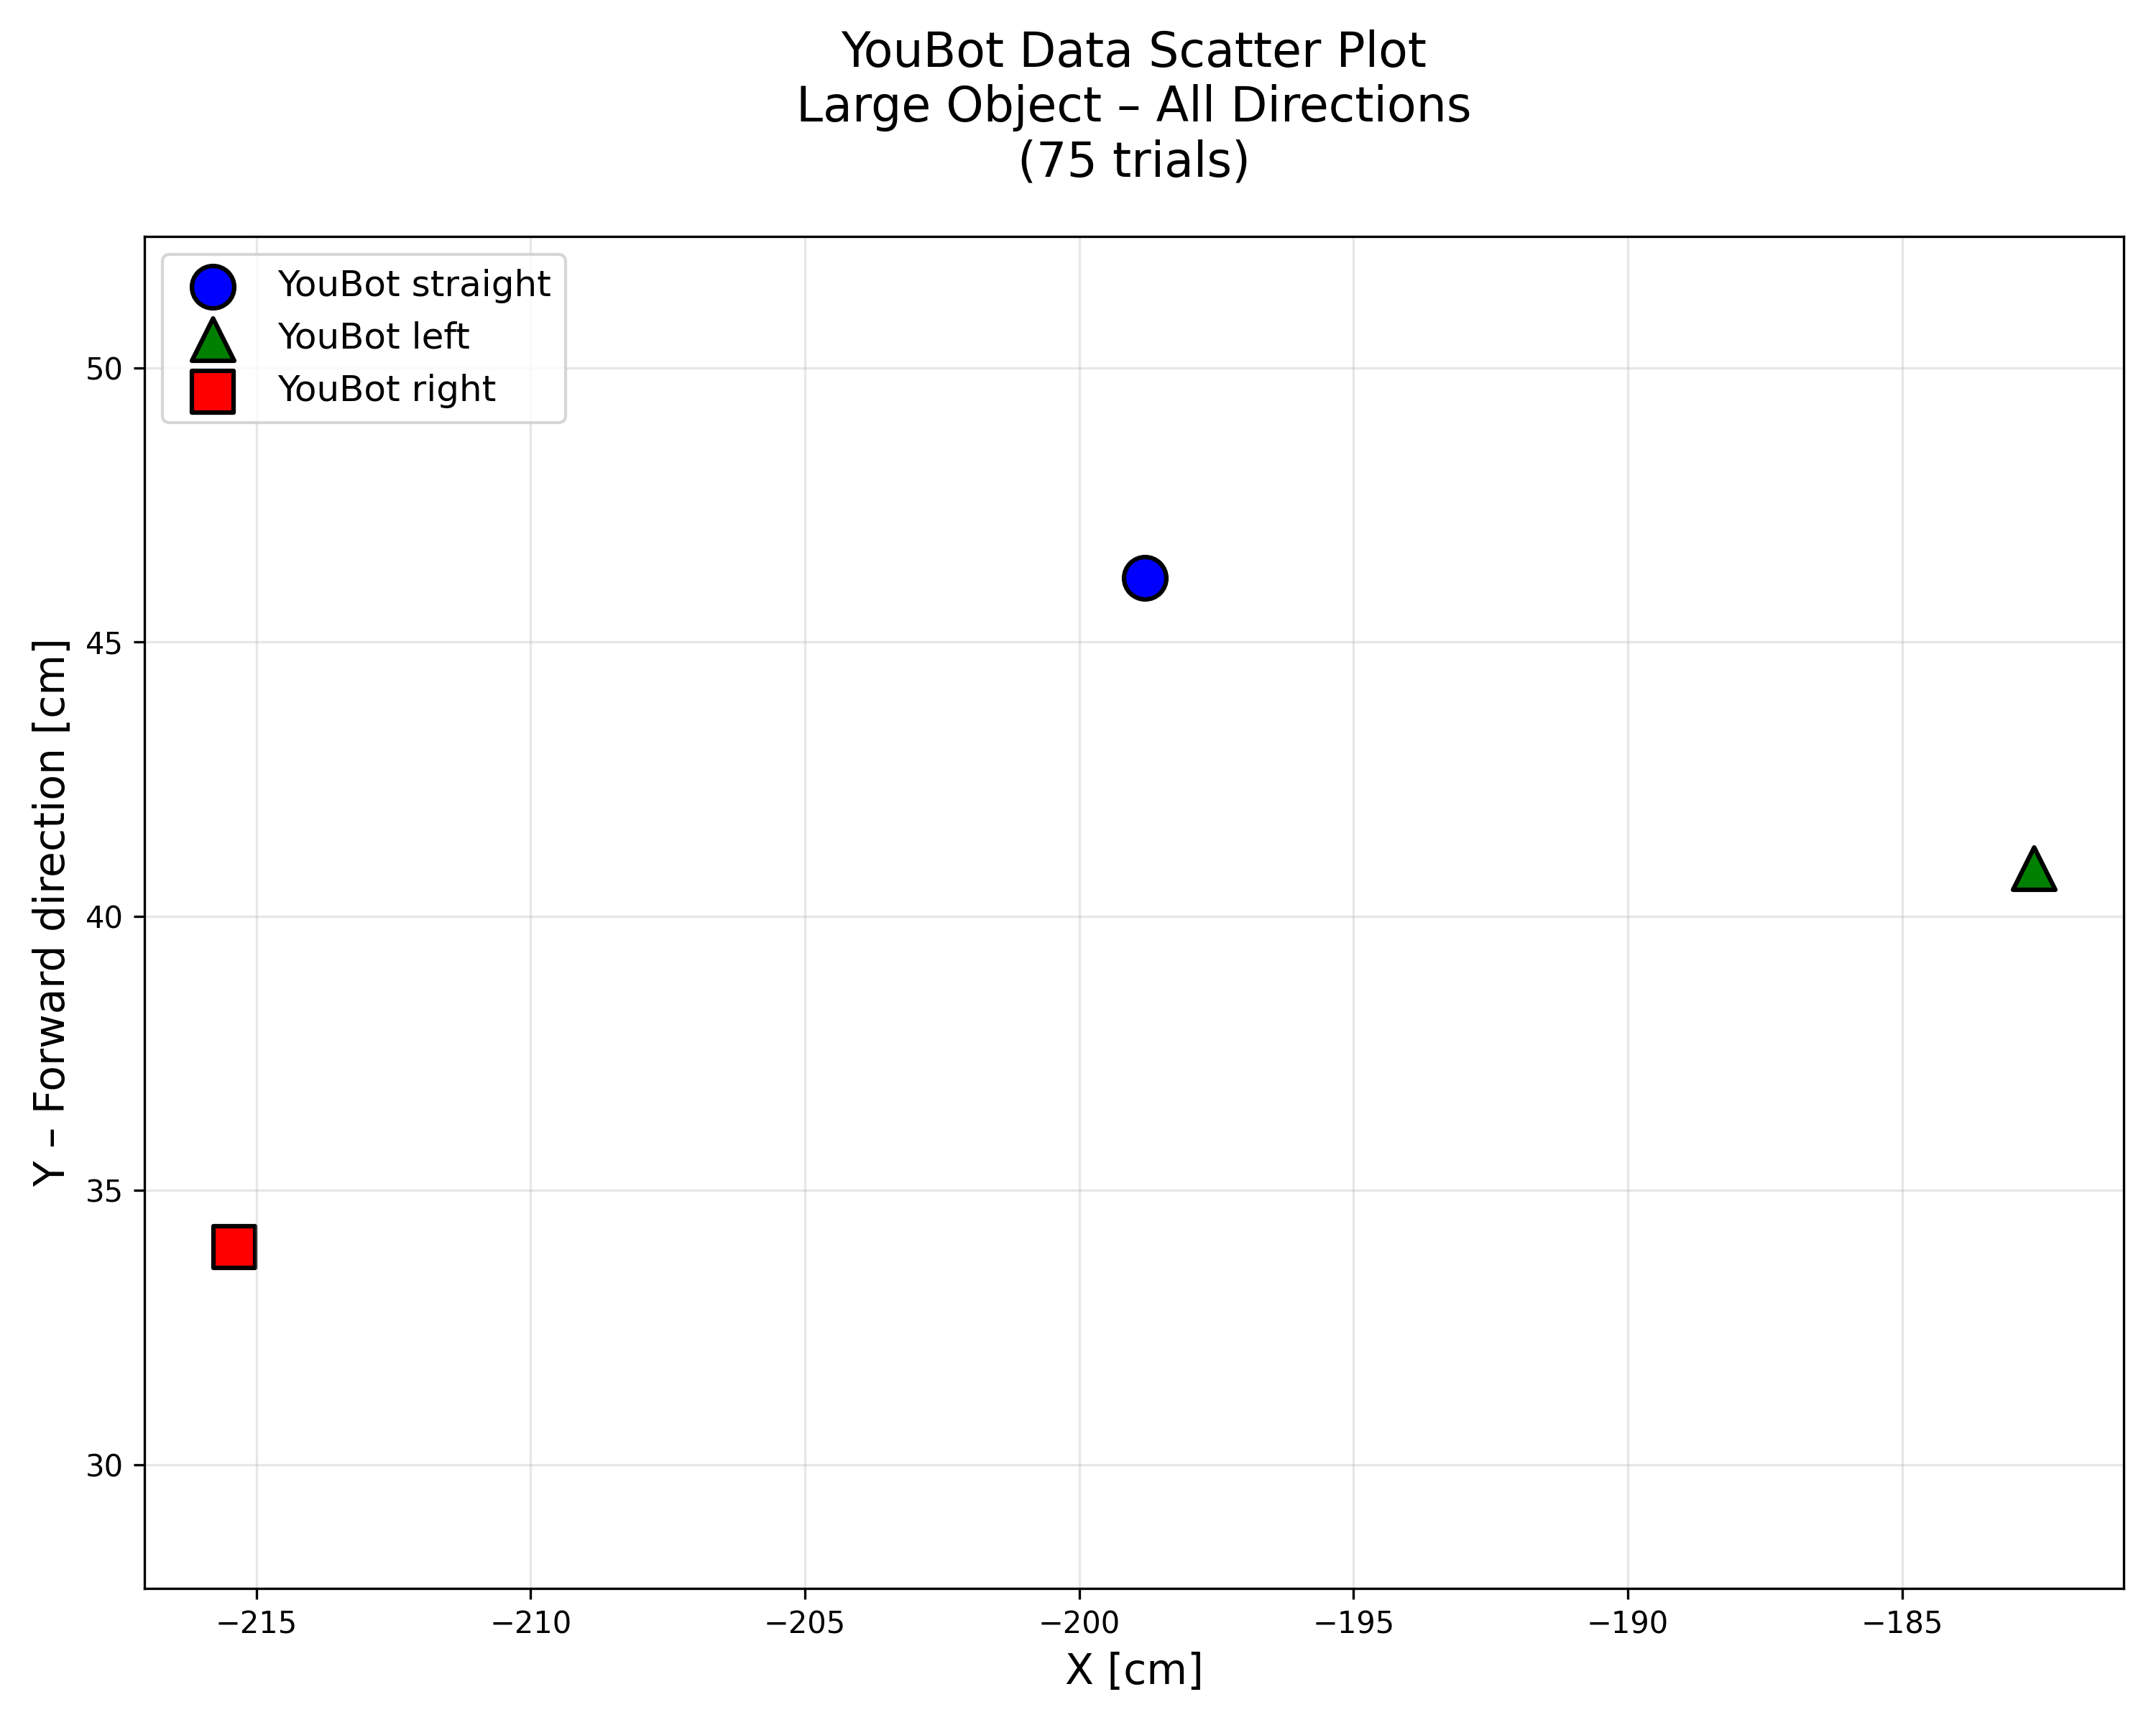
\includegraphics[width=0.8\textwidth]{images/youbot_large.png}
\caption{YouBot Data Scatter Plot for Large Object}
\label{fig:youbot_large}
\end{figure}

\begin{figure}[h!]
\centering
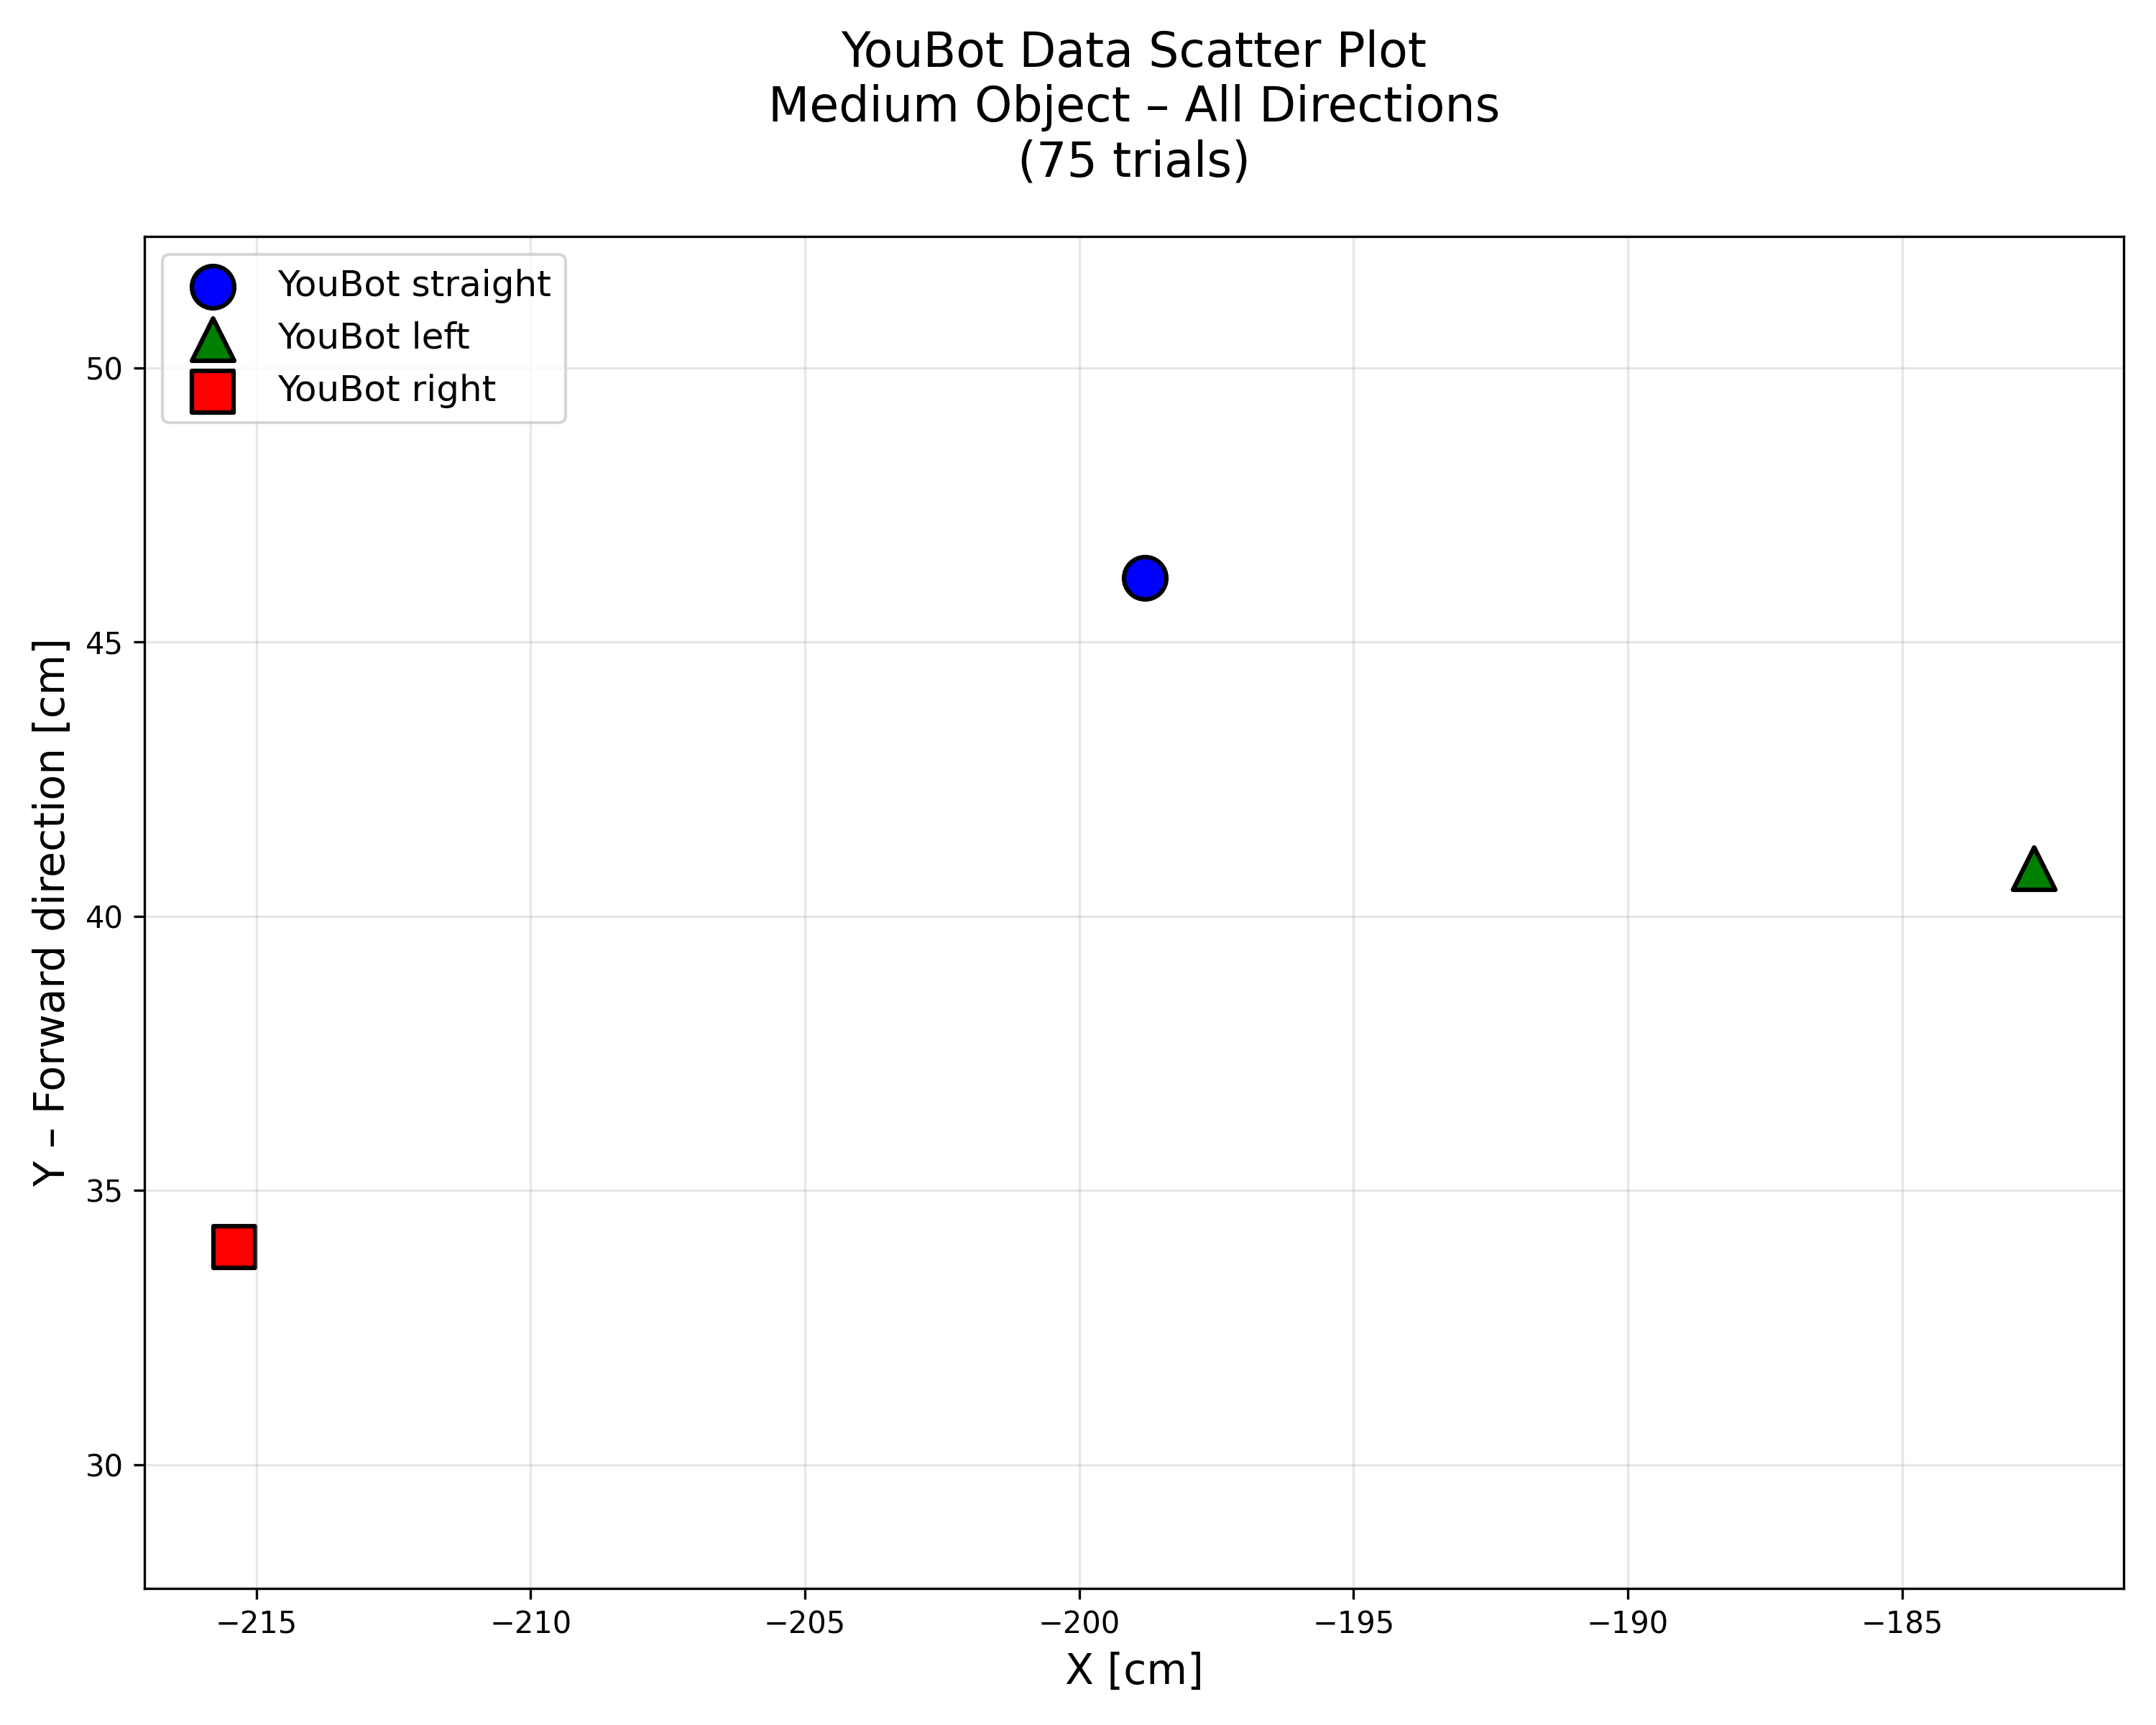
\includegraphics[width=0.8\textwidth]{images/youbot_medium.png}
\caption{YouBot Data Scatter Plot for Medium Object}
\label{fig:youbot_medium}
\end{figure}

\begin{figure}[h!]
\centering
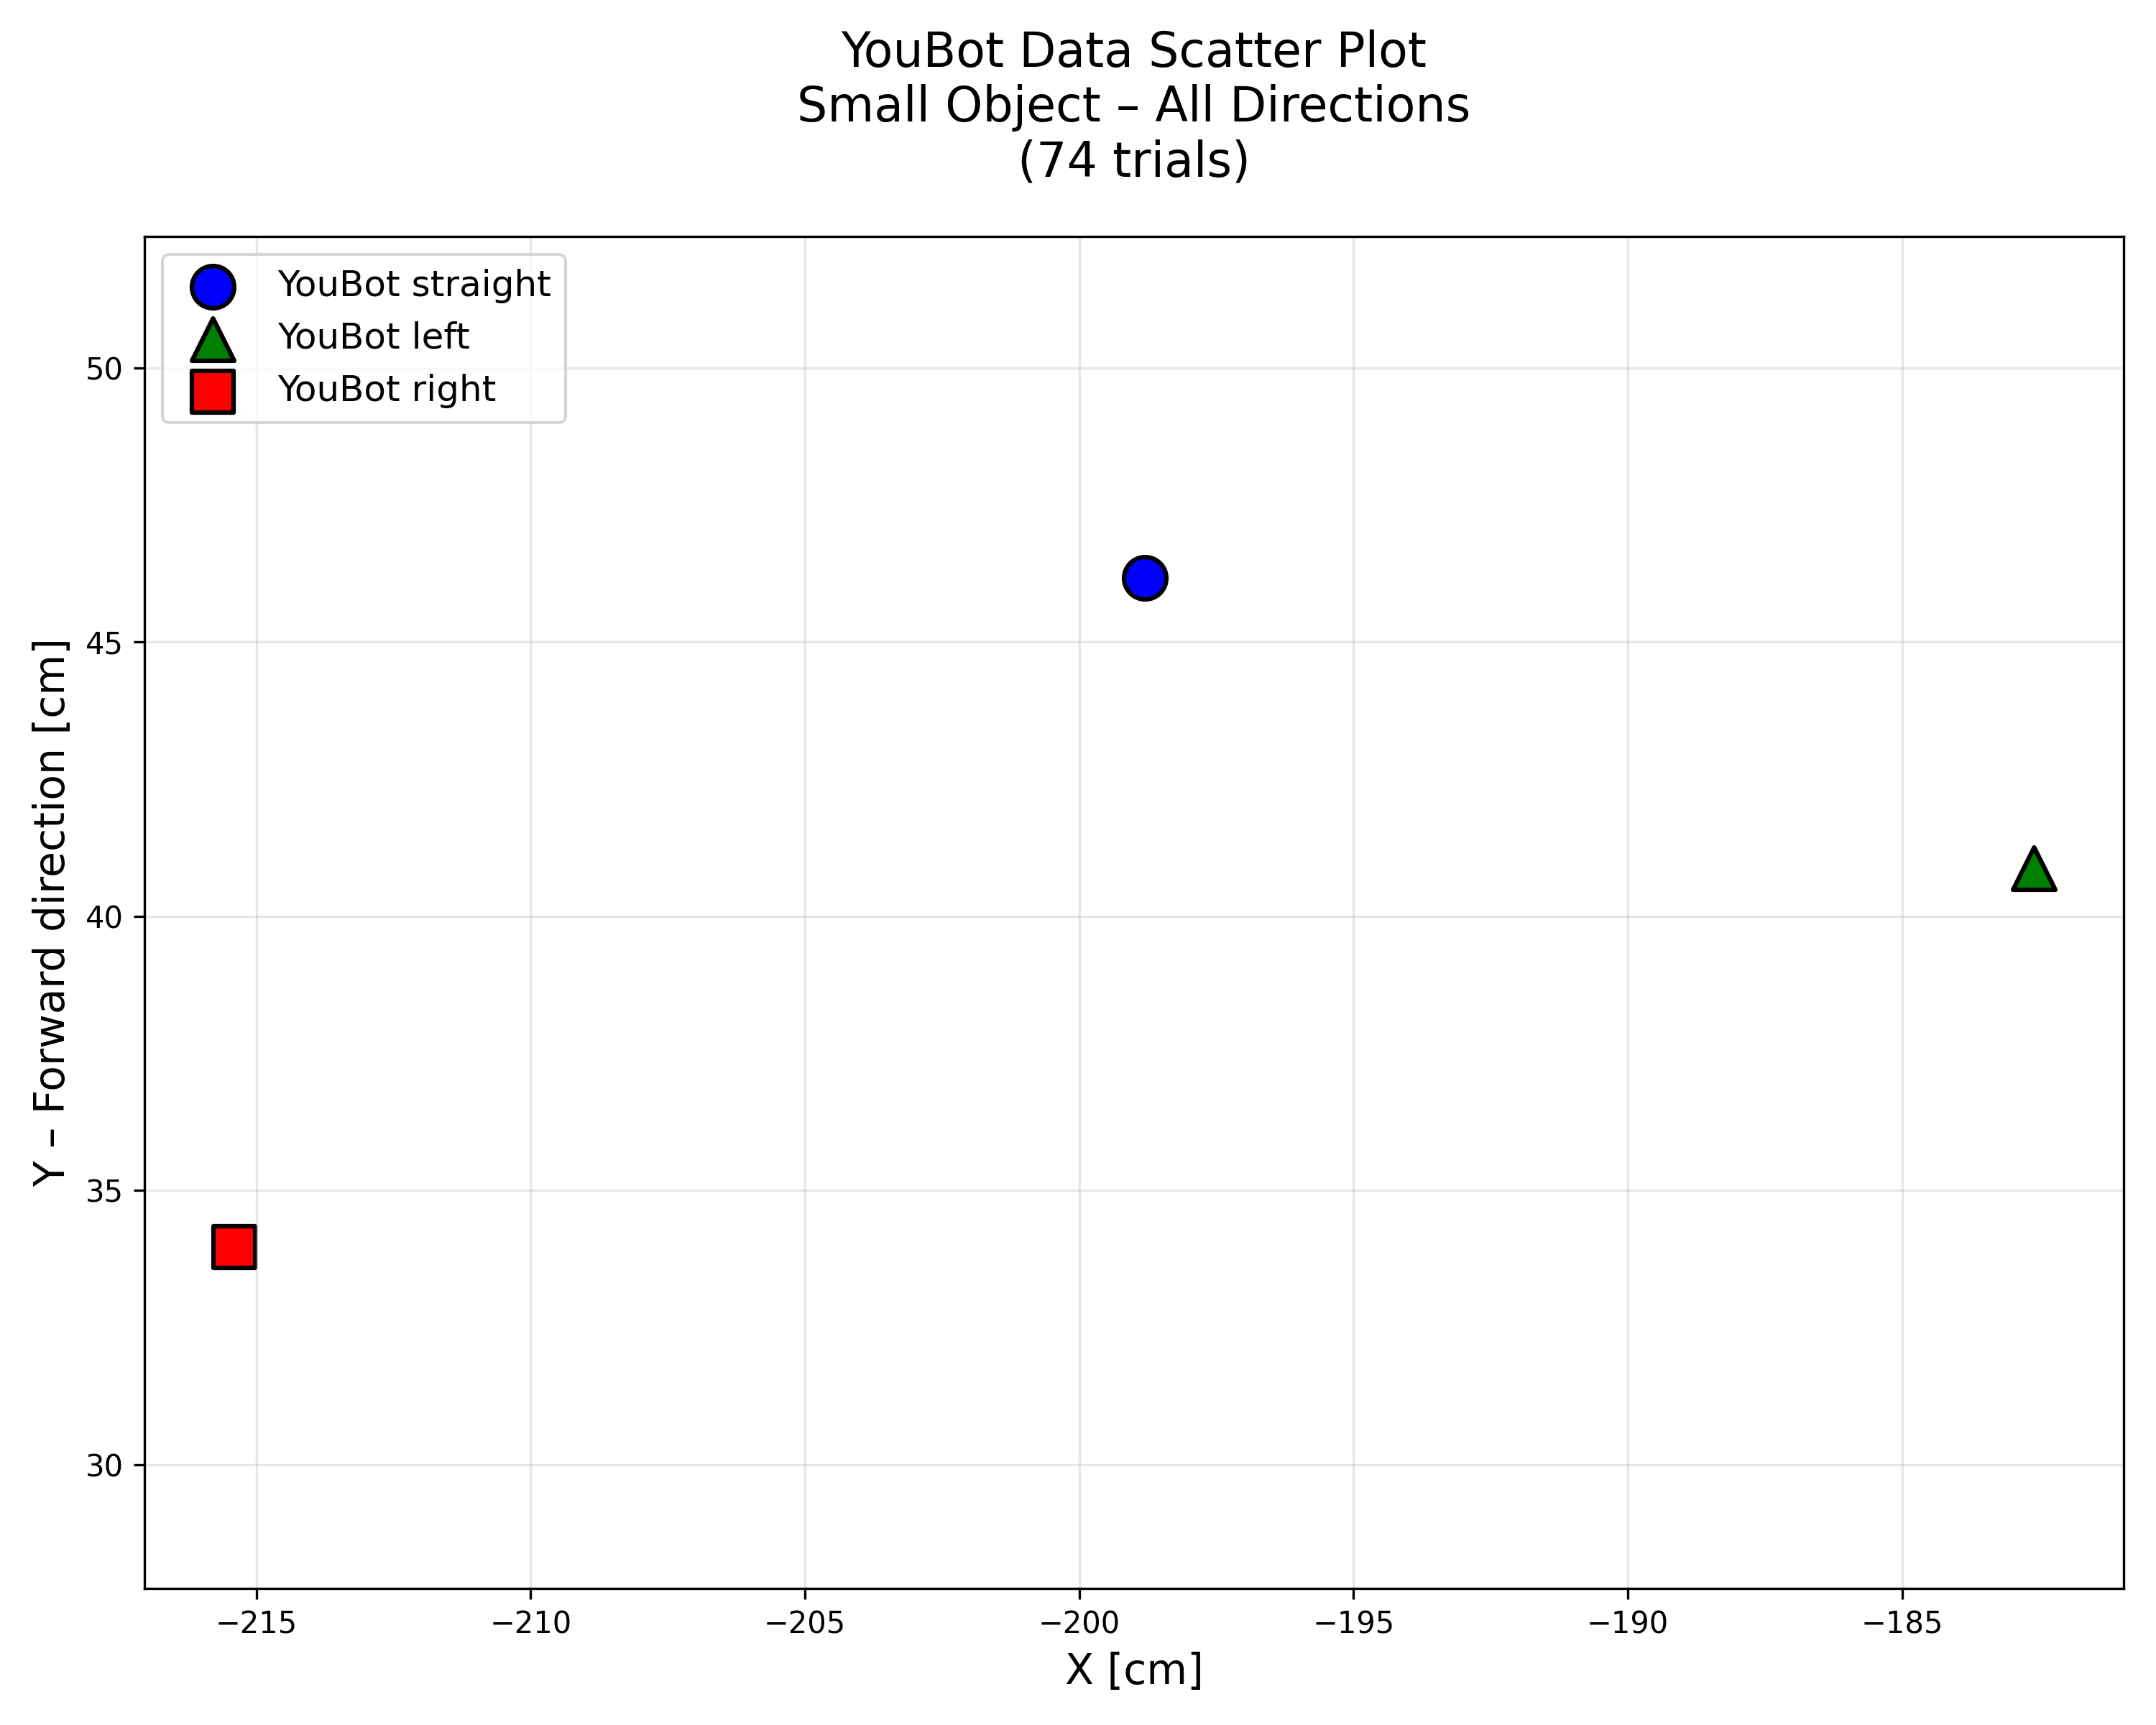
\includegraphics[width=0.8\textwidth]{images/youbot_small.png}
\caption{YouBot Data Scatter Plot for Small Object}
\label{fig:youbot_small}
\end{figure}

\subsection{Combined Transformed Data Scatter Plots}

\begin{figure}[h!]
\centering

\includegraphics[width=0.8\textwidth]{images/combined_large.png}
\caption{Combined Transformed Data Scatter Plot for Large Object}
\label{fig:combined_large}
\end{figure}

\begin{figure}[h!]
\centering

\includegraphics[width=0.8\textwidth]{images/combined_medium.png}
\caption{Combined Transformed Data Scatter Plot for Medium Object}
\label{fig:combined_medium}
\end{figure}

\begin{figure}[h!]
\centering

\includegraphics[width=0.8\textwidth]{images/combined_small.png}
\caption{Combined Transformed Data Scatter Plot for Small Object}
\label{fig:combined_small}
\end{figure}

\section{Conclusion}

After transforming YouBot coordinates to the OptiTrack frame, the KUKA youBot arm demonstrates accuracy ranging from 41.75 to 61.74 cm across object sizes and directions. Precision is high, with standard deviations below 0.14 cm for OptiTrack measurements. Smaller objects show better accuracy, and straight directions exhibit higher precision than lateral movements. The coordinate alignment enables direct comparison of internal and external measurements, providing insights into robot performance for manipulation tasks.